\subsection{超越基}

命题4. --- 设E是域K的扩域，S和T是E的两个子集。则以下性质等价：

\begin{enumerate}
\def\labelenumi{\alph{enumi})}
\item
  \(\mathbf{S} \cup \mathbf{T}\) 是代数自由的（在 \(\mathbf{K}\) 上），且 \(\mathbf{S} \cap \mathbf{T} = \emptyset\) 。
\item
  S 在 K 上代数自由，且 T 在 K(S) 上代数自由。
\item
  T 在 K 上代数自由，且 S 在 K(T) 上代数自由。
\end{enumerate}

显然，只需证明 \(a)\) 与 \(b)\) 等价。

\(a) \Rightarrow b)\) ：假设 \(a)\) 成立。由于 S 包含于 S \(\cup\) T，它在 K 上代数自由。若 T 在 K(S) 上不是代数自由的，则存在（命题3）T 的不同元素的一个有限族 \((y_j)_{1 \leq j \leq n}\) ，它在 K(S) 上代数相关。于是存在一个非零多项式 \(f\) ，在环 K(S) {[}Y \(_1\) , \ldots, Y \(_n\) {]} 中，使得 \(f(y_1, ..., y_n) = 0\) ；必要时把 \(f\) 乘以 K{[}S{]} 的一个非零元素，我们可设 \(f\) 的所有系数都属于 K{[}S{]}。 \(f\) 的系数是 S 的有限多个不同元素 \(x_i\) （ \(1 \leq i \leq m\) ）的、系数在 K 中的多项式。元素 \(x_1, ..., x_m\) 与 \(y_1, ..., y_n\) 两两不同，因为 S \(\cap\) T = ∅。于是关系 \(f(y_1, ..., y_n) = 0\) 可以写成

\[
g \left(x _ {1}, \dots , x _ {m}; y _ {1}, \dots , y _ {n}\right) = 0,
\]

其中 \(g\) 是 \(\mathbf{K}[\mathbf{X}_1, \ldots, \mathbf{X}_m, \mathbf{Y}_1, \ldots, \mathbf{Y}_n]\) 中的非零多项式，而这样一个关系与 \(\mathbf{S} \cup \mathbf{T}\) 代数自由的假设相矛盾。

\(b) \Rightarrow a)\) ：假设 \(b)\) 成立。首先显然有 \(\mathrm{T} \cap \mathrm{K}(\mathrm{S}) = \emptyset\) ，且 \(a\) 更不用说有 \(\mathrm{S} \cap \mathrm{T} = \emptyset\) 。只需证明：若 \(x_i\) （ \(1 \leqslant i \leqslant m\) ）是 \(\mathrm{S}\) 的数目有限的不同元素，而 \(y_j\) （ \(1 \leqslant j \leqslant n\) ）是 \(\mathrm{T}\) 的数目有限的不同元素，则诸 \(x_i\) 与 \(y_j\) 组成的集合在 \(\mathrm{K}\) 上代数自由（命题3）。考虑一个多项式 \(f \in \mathrm{K}[\mathrm{X}_1, \ldots, \mathrm{X}_m, \mathrm{Y}_1, \ldots, \mathrm{Y}_n]\) ，使得 \(f(x_1, \ldots, x_m, y_1, \ldots, y_n) = 0\) ，并令 \(f = \sum_{\alpha_1 \ldots \alpha_n} \varphi_\alpha \mathrm{Y}_1^{\alpha_1} \ldots \mathrm{Y}_n^{\alpha_n}\) ，其中 \(\varphi_\alpha \in \mathrm{K}[\mathrm{X}_1, \ldots, \mathrm{X}_m]\) ，对所有

\(\alpha = (\alpha_{1}, \ldots, \alpha_{n}) \in \mathbf{N}^{n}\) 。设 \(g = f(x_{1}, \ldots, x_{m}, \mathbf{Y}_{1}, \ldots, \mathbf{Y}_{n})\) ；则 \(g\) 是环 \(\mathbf{K}[\mathbf{S}][\mathbf{Y}_{1}, \ldots, \mathbf{Y}_{n}]\) 中的多项式，且关系 \(f(x_{1}, \ldots, x_{m}, y_{1}, \ldots, y_{n}) = 0\) 可写成 \(g(y_{1}, \ldots, y_{n}) = 0\) 。由于 \(T\) 在 \(\mathbf{K}(\mathbf{S})\) 上代数自由，系数 \(\varphi_{\alpha}(x_{1}, \ldots, x_{m})\) （ \(g\) 的）每一个都为零；由于 \(S\) 在 \(K\) 上代数自由，我们有 \(\varphi_{\alpha} = 0\) ，对所有 \(\alpha \in \mathbf{N}^{n}\) ，从而 \(f = 0\) 。

推论. --- 设 E 是域 K 的一个扩域，S 是 E 的一个在 K 上代数自由的子集。若 \(x \in E\) 在 \(\mathrm{K}(\mathrm{S})\) 上是超越的，则 \(S \cup \{x\}\) 在 K 上代数自由。

命题5. --- 设 E 是域 K 的一个扩域。为使 E 的子集 S 在 K 上代数自由，充要条件是：对每个 \(x \in S\) ，元素 x 在域 \(\mathrm{K}(\mathrm{S} - \{x\})\) 上是超越的。

由命题4，该条件是必要的。

为证明充分性，只需（命题3）证明 S 的不同元素的每个有限序列 \((x_{1},\ldots,x_{n})\) 是代数自由的。由假设， \(x_{i}\) 在 \(\mathrm{K}(x_{1},\ldots,x_{i-1})\) 上是超越的，对 \(1\leqslant i\leqslant n\) ，于是我们的断言由命题4的推论通过对 n 的归纳得出。

命题6. --- 设 E 是域 K 的一个扩域，X 是 E 的在 K 上代数自由的一个子集。若 \(K' \subset E\) 是 K 的一个代数扩张，则 X 在 \(K'\) 上代数自由。

用反证法，假设 X 在 \(K'\) 上代数相关。由命题5，存在一个元素 \(x \in X\) ，它在域 \(\mathbf{K}'(\mathbf{M})\) 上是代数的，其中 \(\mathbf{M} = \mathbf{X} - \{x\}\) 。由于 \(\mathbf{K}'(\mathbf{M}) = \mathbf{K}(\mathbf{M})(\mathbf{K}')\) 且 \(K'\) 在 K 上代数，V 第18页推论2表明 \(\mathbf{K}'(\mathbf{M})\) 在 \(\mathbf{K}(\mathbf{M})\) 上是代数的；由于 x 在 \(\mathbf{K}'(\mathbf{M})\) 上代数，因此它在 \(\mathbf{K}(\mathbf{M}) = \mathbf{K}(\mathbf{X} - \{x\})\) 上是代数的，由 V 第19页命题3。现在命题5表明 X 在 K 上代数相关，遂得矛盾。

定义3. --- 域 K 的扩域 E 的子集 B 称为 E（在 K 上）的超越基，如果 B 在 K 上代数自由，且 E 在 K(B) 上是代数的。

\pandocbounded{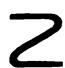
\includegraphics[keepaspectratio]{images/part002_88480e13.jpg}}

例. --- 纯基是超越基。另一方面，若 E 是 K 的一个纯扩张，E 在 K 上的一个超越基不总是 E 的纯基。例如，在 \(\mathbf{K}(\mathbf{X})\) 中， \(\{\mathbf{X}^{2}\}\) 是一个超越基，但不生成 \(\mathbf{K}(\mathbf{X})\) 。

命题7. --- 设 E 是域 K 的一个扩域。 E 的每个超越基都是 E 的在 K 上代数自由的子集所成集合（按包含关系排序）中的极大元。反之，若 S 是 E 的一个子集，使得 E 在 K(S) 上是代数的，则 S 的每个极大代数自由子集都是 E 的一个超越基。

设 B 是 E 在 K 上的一个超越基，且 \(x \in E - B\) 。则 x 在 \(\mathrm{K}(\mathrm{B})\) 上是代数的；由 V 第107页命题4，E 的子集 \(B \cup \{x\}\) 在 K 上不是代数自由的，由此得命题的第一部分。其次，若 E 在 \(\mathrm{K}(\mathrm{S})\) 上代数，且 B 是 S 的一个极大代数自由部分，则由命题4的推论，每个 \(x \in S\) 在 \(\mathrm{K}(\mathrm{B})\) 上是代数的；于是（V，第18页，推论1） \(\mathrm{K}(\mathrm{S})\) 在 \(\mathrm{K}(\mathrm{B})\) 上是代数的，从而（V，第19页，命题3）E 在 \(\mathrm{K}(\mathrm{B})\) 上是代数的。

定理1（施泰尼茨）。--- 域 K 的每个扩域 E 在 K 上都拥有一个超越基。换言之，域 K 的每个扩张都是 K 的一个纯扩张的代数扩张。

\pandocbounded{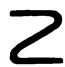
\includegraphics[keepaspectratio]{images/part002_71d10db7.jpg}}

相反，一个扩张并不总是代数扩张的纯扩张（V，第171页，习题2）。

此定理是以下更精确结果的一个推论：

定理2. --- 设 E 是域 K 的一个扩域，S 是 E 的一个使 E 在 K(S) 上代数的子集，T 是 S 的一个在 K 上代数自由的子集；则存在 E 在 K 上的一个超越基 B，使得 \(T \subset B \subset S\) 。

因为 S 的代数自由子集所成的集合按包含关系排序，由命题3是一个有限特征集（E，III，第34页）。由 E，III，第35页的定理1，它有一个包含 T 的极大元 B，且由命题7，B 是 E 在 K 上的一个超越基。

推论（«交换定理»）。--- 设 E 是 K 的一个扩域，S 是 E 的一个使 E 在 K(S) 上代数的子集，T 是 E 的一个在 K 上代数自由的子集；则存在 S 的一个子集 S'，使得 T ∪ S' 是 E 在 K 上的一个超越基，且 T ∩ S' = ∅。

因为 E 在 \(\mathbf{K}(\mathbf{T} \cup \mathbf{S})\) 上是代数的，且我们有 \(T \subset T \cup S\) 。

